\documentclass{article}
% Problems faithfully transcribed from Problem Set 3.pdf.
\usepackage[en]{homework}
\usepackage{tikz}
\usetikzlibrary{patterns}

\config{Physics-1}{2026 秋季}{3}

\begin{document}

\begin{problem}
A commonly used potential energy function to describe the interaction between two atoms is the Lennard-Jones 6-12 potential given by
\[
  U=\epsilon\left[\left(\frac{r_0}{r}\right)^{12}-2\left(\frac{r_0}{r}\right)^6\right]
\]
\begin{enumerate}
  \item[a)] Find the position of the potential minimum and its value.
  \item[b)] Near the minimum the atoms execute simple harmonic motion. Find the frequency of oscillation.
\end{enumerate}
\end{problem}

\begin{problem}
\textit{Sand and conveyor belt}

Sand runs from a hopper at constant rate $dm/dt$ onto a horizontal conveyor belt driven at constant speed $V$ by a motor.
\begin{center}
  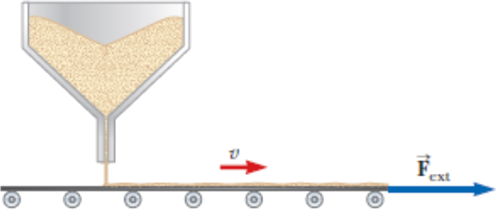
\includegraphics[width=0.55\linewidth]{sand-conveyor.png}
\end{center}
\begin{enumerate}
  \item[(a)] Find the power needed to drive the belt.
  \item[(b)] Compare the answer to (a) with the rate of change of kinetic energy of the sand. Can you account for the difference?
\end{enumerate}
\end{problem}

\begin{problem}
A block of mass $M$ on a horizontal frictionless table is connected to a spring (spring constant $k$). The block is set in motion so that it oscillates about its equilibrium point with a certain amplitude $A_0$. The period of motion is $T_0=2\pi\sqrt{M/k}$.
\begin{enumerate}
  \item[(a)] A lump of sticky putty of mass $m$ is dropped onto the block. The putty sticks without bouncing. The putty hits $M$ at the instant when the velocity of $M$ is zero. Find
  \begin{enumerate}
    \item[(1)] The new period.
    \item[(2)] The new amplitude.
    \item[(3)] The change in the mechanical energy of the system.
  \end{enumerate}
  \item[(b)] Repeat part (a), but this time assume that the sticky putty hits $M$ at the instant when $M$ has its maximum velocity.
\end{enumerate}
\end{problem}

\begin{problem}
A light particle of mass $m$ is placed at rest ($v_0=0$) on a frictionless floor, facing a wall. A heavy particle of mass $M$ collides at speed $V_0$ on the particle of mass $m$. After the collision, the light particle is shot leftward, collides on the wall and bounces back. Then, the light particle collides on the heavy particle (which is still moving leftward) and bounces back. Then, the light particle collides on the wall and bounces back... It continues to bounce back and forth in this manner until the heavy particle moves rightward at speed larger than the rightward speed of the light particle. All collisions are elastic. For $m=1$ kg and $M=100$ kg, there are 31 collisions. (See the video clip posted online along with the exercise.)
\begin{center}
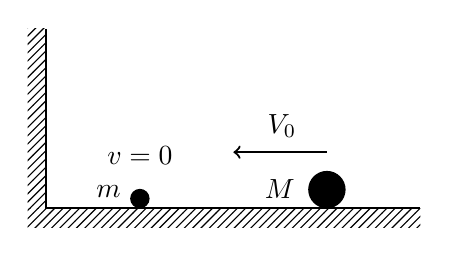
\begin{tikzpicture}[scale=0.95, line width=0.7pt]
  \fill[pattern=north east lines] (-0.25,0) rectangle (0,2.4);
  \fill[pattern=north east lines] (-0.25,-0.25) rectangle (5,0);
  \draw[thick] (0,2.4) -- (0,0) -- (5,0);
  \fill (1.25,0.13) circle (0.13);
  \fill (3.75,0.25) circle (0.25);
  \node at (0.83,0.22) {$m$};
  \node at (3.12,0.26) {$M$};
  \node at (1.25,0.7) {$v=0$};
  \draw[->,thick] (3.75,0.75) -- (2.5,0.75);
  \node at (3.15,1.1) {$V_0$};
\end{tikzpicture}
\end{center}
\begin{enumerate}
  \item[(a)] Let $v$ be the velocity of mass $m$ and $V$ be the velocity $M$. Suppose we have $V=V(n)$ and $v=v(n)$ after the mass $m$ collides with $M$ and the wall $n$ times. We have $V(0)=V_0$ and $v(0)=0$. Using momentum conservation and energy conservation, write down two equations that relate $(v(1),V(1))$ and $(v_0,V_0)$.
  \item[(b)] Introduce variables $X=cv$ and $Y=CV$ for some constants $c$ and $C$ such that the points $(v_0,V_0)$ and $(v(1),V(1))$ are on the unit circle $X^2+Y^2=1$. Plot on this circle the point $(v(2),V(2))$, determined by the velocities of the masses right after $m$ hits the wall for the first time.
  \item[(c)] Give a rough plot of the subsequent points $(X(n),Y(n))$ corresponding to $(v(n),V(n))$, $n=3,4,\ldots$, on the circle $X^2+Y^2=1$.
  \item[(d)] For $\theta\ll1$, we have $\arctan\theta\approx\theta$. What is the total number of collisions when $m=1$ kg and $M=100,000,000$ kg?
\end{enumerate}
\end{problem}

\newpage
\begin{problem}
A chain of mass $M$ and length $l$ is suspended vertically with its lowest end touching a scale. The chain is released and falls onto the scale. What is the reading of the scale when a length of chain, $x$, has fallen? (Neglect the size of individual links.)
\begin{center}
  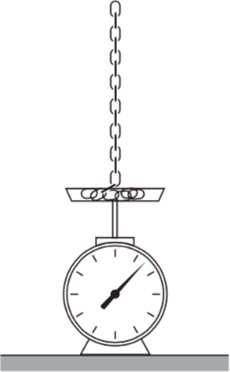
\includegraphics[width=0.23\linewidth]{chain-scale.png}
\end{center}
\end{problem}

\end{document}
